{\color{red}{[DEFINE INCREMENT VERSUS TENDENCY CLEARLY; STRAIGHTEN OUT NOTATION FOR CSLAM GRID AND PG3 - ALSO IN FIGURES]}}\\

Separating dynamics, tracer and physics grids introduces the added complexity of having to map the state from dynamics and tracer grids to the physics grid; and mapping physics tracer increments back to the tracer grid and physics increments needed by the dynamical core to the dynamics grid. The dynamics grid refers to the Gauss-Lobatto-Legendre (GLL) quadrature nodes used by the spectral-element method to solve the momentum equations for the momentum vector $(u,v)$, thermodynamics equation for temperature ($T$), continuity equation for dry air ($p$), and continuity equations for water vapor and condensates thermodynamically active \citep[see, e.g., ][ for details]{LetAl2018JAMES}. By tracer grid we refer to the $pg3$ grid on which CSLAM performs tracer transport of water vapor, condensates and other tracers. The GLL value for water vapor and condensates is overwritten by the CSLAM values every physics time-step so that the spectral-element advection of water species does not become decoupled from the the CSLAM advection of the same water species. Mapping velocity components, dry air mass and temperature from the GLL grid to the $pg2$ grid is done by using the internal degree 3 Lagrange basis functions in CAM-SE \citep[as described in  ][ for pg3; exactly the same methods can be used for $pg2$]{HL2018MWR}.

As compared to the $pg3$ configuration, the extra complication of the $pg2$ setup is that tracer state needs to be mapped from the tracer grid to the physics grid and tracer increments from physics need to the mapped from the physics grid to CSLAM grid. In order to describe the algorithm some notation needs to be introduced.

The mapping algorithm is applied to each element $\Omega$ (with spherical area $\Delta \Omega$) so without loss of generality consider one element. Let $\Delta A^{(pg)}_k$ and $\Delta A^{(nc)}_\ell$ be the spherical area of the physics grid cell $A^{(pg)}_k$ and CSLAM control volume $A^{(nc)}_\ell$, respectively. The physics grid cells and CSLAM cells respectively span the element without gaps or overlaps
\begin{eqnarray}
\cup_{k=1}^{pg^2}A^{(pg)}_k=\Omega \text{ and } A^{(pg)}_k \cap A^{(pg)}_\ell = \emptyset \quad \forall k\ne \ell,\\
\cup_{k=1}^{nc^2}A^{(nc)}_k=\Omega \text{ and } A^{(nc)}_k \cap A^{(nc)}_\ell = \emptyset \quad \forall k\ne \ell.
\end{eqnarray}
The overlap areas between the $k$-th physics grid cell and CSLAM cells is denoted
\begin{equation}
A_{k\ell}=A^{(pg)}_k \cap A^{(nc)}_\ell,
\end{equation}
(see Figure \ref{fig:area-schematic}) so that
\begin{equation}
A^{(pg)}_k=\cup_{l=1}^{nc^2}A_{k\ell}.
\end{equation}
This overlap grid is also referred to as an exchange grid.
\subsection{Mapping tracers from $A^{(nc)}$ to $A^{(pg)}$ (CSLAM to physics grid)}\label{sec:nctopg}
The CSLAM and physics grids are both finite-volume grids so exising CSLAM technology can be used, i.e. perform a high-order shape-preserving reconstruction of mixing ratio $m$ and dry air mass  $\frac{1}{g}\Delta p$ inside each CSLAM control volume and integrate those reconstruction functions over the overlap areas \citep{LNU2010JCP,NL2010JCP}. This algorithm retains the properties of CSLAM: inherent mass-conservation, consistency (constant mixing ratio is preserved), mixing ratio shape-preservation and linear-correlation preservation. 

In mathematical terms, the dry pressure level thickness integrated over the $k$'th physics grid cell is given by
\begin{equation}
\overline{\Delta p}^{(pg)}_k=\sum_{\ell=1}^{nc^2}\langle \Delta p\rangle_{k\ell},
\end{equation}
where $\langle \Delta p\rangle_{k\ell}$ is the integral over the high-order reconstruction of $\Delta p$ over the overlap area $A_{k\ell}$ divided by the area of the overlap
\begin{equation}
\langle \Delta p\rangle_{k\ell}=\frac{1}{\delta A_{k\ell}}\int_{A_{k\ell}}\left[ \sum_{i+j\le 2}{\mathcal{P}}^{(ij)}_\ell x^{i}y^{j}\right] dA,
\end{equation}
where the reconstruction coefficients ${\mathcal{P}}^{(ij)}_\ell$ in CSLAM cell $\ell$ are computed from the cell average pressure level thicknesses on the CSLAM grid $\Delta p^{(nc)}$ and the numerical integration over overlap areas is done by line-integral quadrature. The details are given in \cite{LNU2010JCP} and not repeated here.

The tracer mass per unit area on the physics grid is given by
\begin{equation}
\label{eq:mp}
\overline{m\Delta p}^{(pg)}_k=\sum_{\ell=1}^{nc^2}\langle m\Delta p\rangle_{k\ell},
\end{equation}
where $\langle m\Delta p\rangle_{k\ell}$ is the integral over the high-order reconstruction of $\Delta p$ and $m$ combined using the approach outlined in Appendix B of \cite{NL2010JCP} over the overlap area $A_{k\ell}$
\begin{equation}
\label{eq:mp2}
\langle m\Delta p\rangle_{k\ell}=\frac{1}{\delta A_{k\ell}}\int_{A_{k\ell}}\left[ \overline{\Delta p}_\ell^{(nc)}\sum_{i+j\le 2}{\mathcal{M}}^{(ij)}_\ell x^{i}y^{j}+{\overline{m}}_\ell^{(nc)}\sum_{i+j\le 2}{\widetilde{{\mathcal{P}}}}^{(ij)}_\ell x^{i}y^{j}\right] dA,
\end{equation}
where ${\widetilde{{\mathcal{P}}}}^{(00)}_\ell={\mathcal{P}}^{(00)}_\ell-\overline{\Delta p}^{(nc)}_\ell$ and ${\widetilde{{\mathcal{P}}}}^{(ij)}_\ell={\mathcal{P}}^{(ij)}_\ell$ for $i,j>0$, and ${\mathcal{M}}^{(ij)}_\ell$ are the reconstruction coefficients for the mixing ratio in CSLAM cell $A^{(nc)}_\ell$. The mixing ratio on the physics grid is then
\begin{equation}
\overline{m}^{(pg)}_k=\frac{\overline{m\Delta p}^{(pg)}_k}{\overline{\Delta p}^{(pg)}_k}.
\end{equation}
It has been demonstrated in  \cite{LNU2010JCP} that this mapping algorithm exhibits the properties outlined above and hence not repeated here. A much more challenging problem is to map tracer increments from the physics grid to the CSLAM grid while retaining important properties.
\subsection{Mapping tracer increments from $A^{(pg)}$ to $A^{(nc)}$ (physics to CSLAM grid)}\label{sec:pgtonc}
The increments from the parameterizations are computed on the physics grid. The tracer increment in physics grid cell $k$ is denoted $f_k^{(pg)}$ so that the updated mixing ratio on the physics grid is $m^{(pg)}_k+f_k^{(pg)}$. The problem is how to map $f_k^{(pg)}$ to the CSLAM control volumes $f^{(nc)}$ satisfying the following constraints:
\begin{enumerate}
\item {\bf{Local mass-conservation}}: Total physics mass forcing on an element computed on the physics grid should equal the element physics mass forcing on the CSLAM grid
\begin{equation}
f_k^{(pg)}\Delta p^{(pg)}_k\Delta A_k^{(pg)}=\cup_{\ell=1}^{nc^2}\Delta A_{k\ell}\Delta p^{(nc)}_\ell f^{(nc)}_\ell,
\end{equation}
where $\Delta p^{(pg)}_k$ is the pressure level thickness in physics grid cell $k$ and similarly for $\Delta p^{(nc)}$.
\item {\bf{Shape-preservation in mixing ratio}}: The increments mapped to the CSLAM grid and added to the previous CSLAM state should not produce values smaller than the updated physics grid mixing ratios, $m^{(pg)}_k+f_k^{(pg)}$, or values smaller than the existing CSLAM mixing ratios
\begin{equation}
m^{(min)}=\min \left( m^{(pg)}_k+f_k^{(pg)},\left\{ m^{(nc)}_{\ell} |\ell=1,nc^2\right\} \right),
\end{equation}
Similarly for maxima
\begin{equation}
m_k^{(max)}=\max \left( m^{(pg)}_k+f_k^{(pg)},\left\{ m^{(nc)}_{k\ell} |\ell=1,nc^2\right\} \right),
\end{equation}
\item {\bf{Linear correlation preservation}}: The physics forcing must not disrupt linear tracer correlation between species on the CSLAM grid \citep[see, e.g., ][]{LT2011QJR}.
\item {\bf{Consistency}}: A constant mixing ratio increment from physics, $cnst$, on the physics grid, $f_k^{(pg)}=cnst$ $\forall k$, must result in the same (constant) forcing on the CSLAM grid, $f_\ell^{(nc)}=f_k^{(pg)}=cnst$ $\forall \ell$.
\end{enumerate}
To motivate the algorithm that will simultaneously satisfy 1-4 it is informative to discuss how `standard' mapping algorithms will violate one or more of the constraints:
\subsubsection{Why conservative remapping won't work!}
It is helpful to analyze in detail why conventional remapping can not satisfy properties 1-4 above. Assume that one remaps the mass-increments in exactly the same way as the mapping of mixing ratio state from the CSLAM grid to the physics grid described in section \ref{sec:nctopg}. That is, replace $m$ with $f$ and map from physics grid to the CSLAM grid instead of the other way around. {\color{red}{explain algorithm with math ... need it for high-order preallocation!}} The mapped mass-increment is $\overline{f\Delta p}^{(pg)}_k$ and due to the properties of the mapping algorithm the mass-increment is conserved, linear correlation between mass-increments are conserved and shape in mass-increment is preserved.

That said, this approach is problematic. The issue is that the dry pressure level thickness mapped from $pg$ to $nc$, call it $\widetilde{\overline{\Delta p}}^{(nc)}$, differs from $\overline{\Delta p}^{(nc)}$. During physics-dynamics coupling the dry pressure level thickness should remain constant. So when converting the mass-increments to mixing ratio increments through, e.g.,
\begin{equation}
\overline{m}^{(pg)}_k=\frac{\overline{f\Delta p}^{(pg)}_k}{\overline{\Delta p}^{(pg)}_k},
\end{equation}
a constant mixing ratio increment is not conserved since $\widetilde{\overline{\Delta p}}^{(pg)}_k\ne {\overline{\Delta p}}^{(pg)}_k$. Basically the constant increment will map to a field representing the spurious discrepancy between $\widetilde{\overline{\Delta p}}^{(pg)}_k$ and ${\overline{\Delta p}}^{(pg)}_k$. A constant increment can be preserved by using
\begin{equation}
\overline{m}^{(pg)}_k=\frac{\overline{f\Delta p}^{(pg)}_k}{\widetilde{\overline{\Delta p}}^{(pg)}_k},
\end{equation}
instead, but now mass-conservation is lost since $\widetilde{\overline{\Delta p}}^{(pg)}_k\ne {\overline{\Delta p}}^{(pg)}_k$. This issue is similar to the mass-wind inconsistency found in specified dynamics applications \citep[e.g.][]{JKLSBCRE2001QJR}. 

\begin{figure}[t]
\begin{center}
\noindent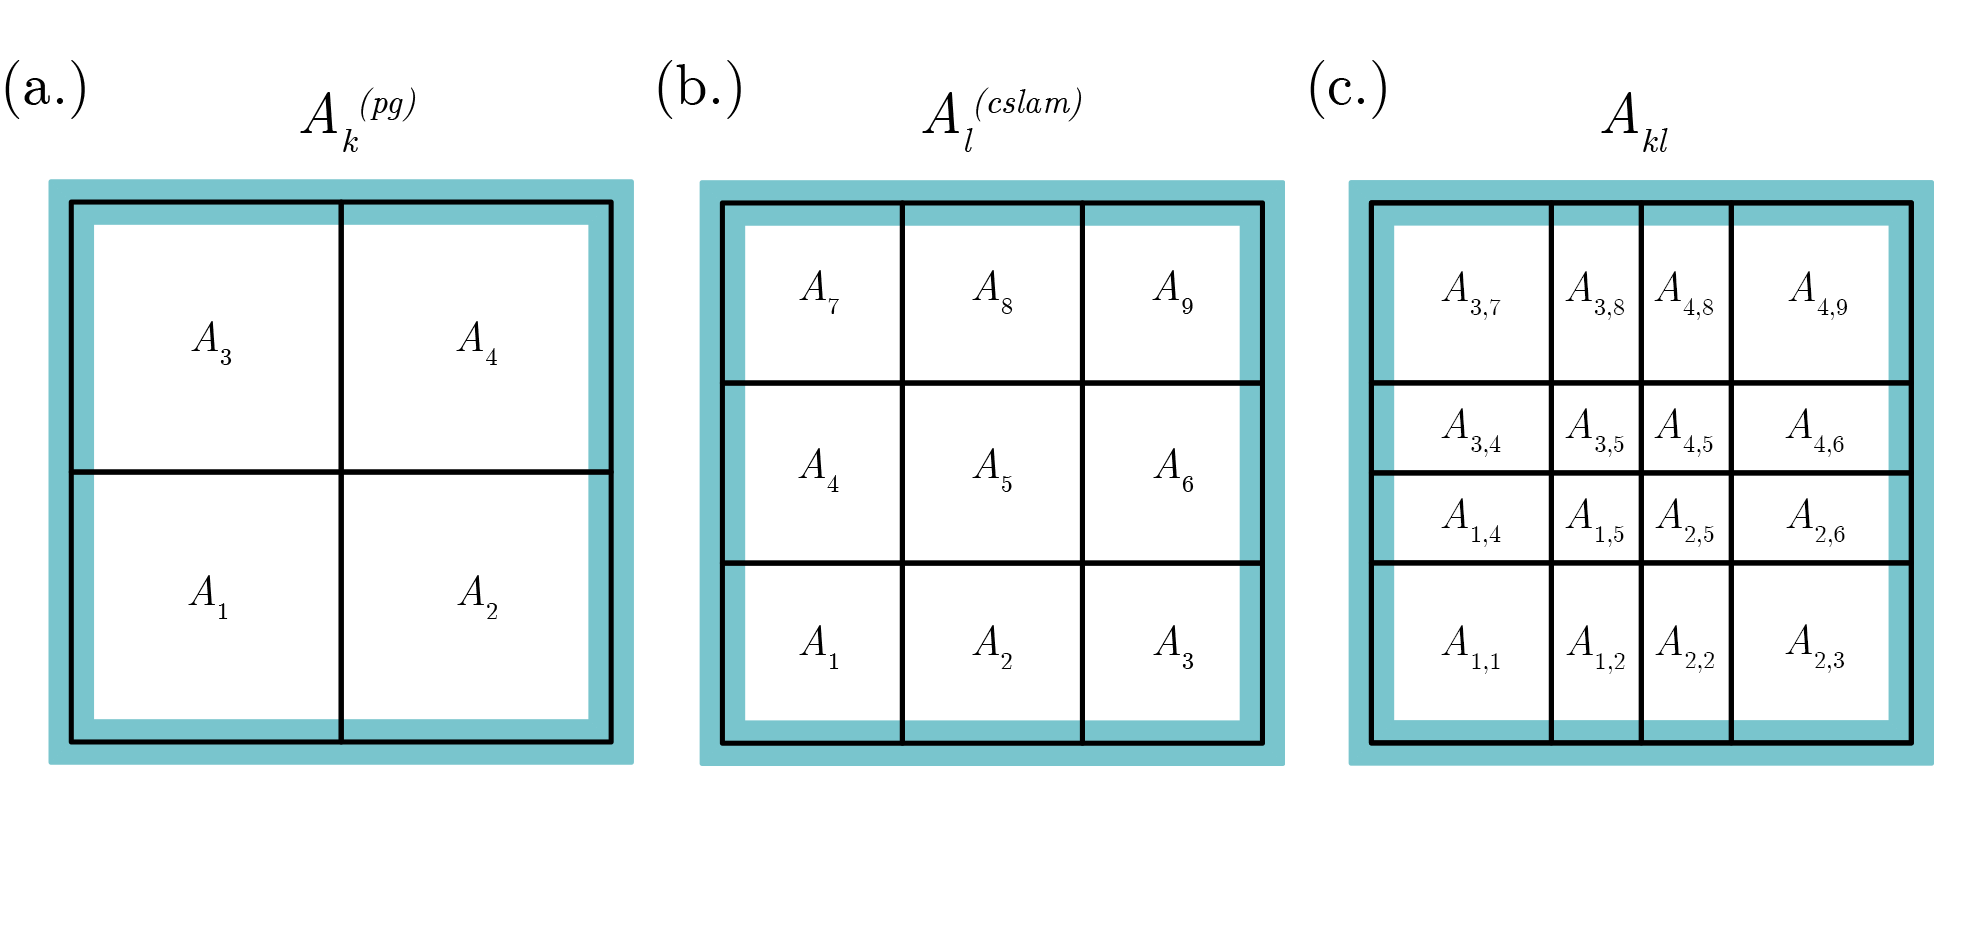
\includegraphics[width=30pc,angle=0]{figs/area-schematic.png}\\
\end{center}
\caption{Indices notation for (a) the $pg2$ grid, (b) the $pg3$ grid and (c) their exchange grid.}
\label{fig:area-schematic}
\end{figure}

\begin{figure}[t]
\begin{center}
\noindent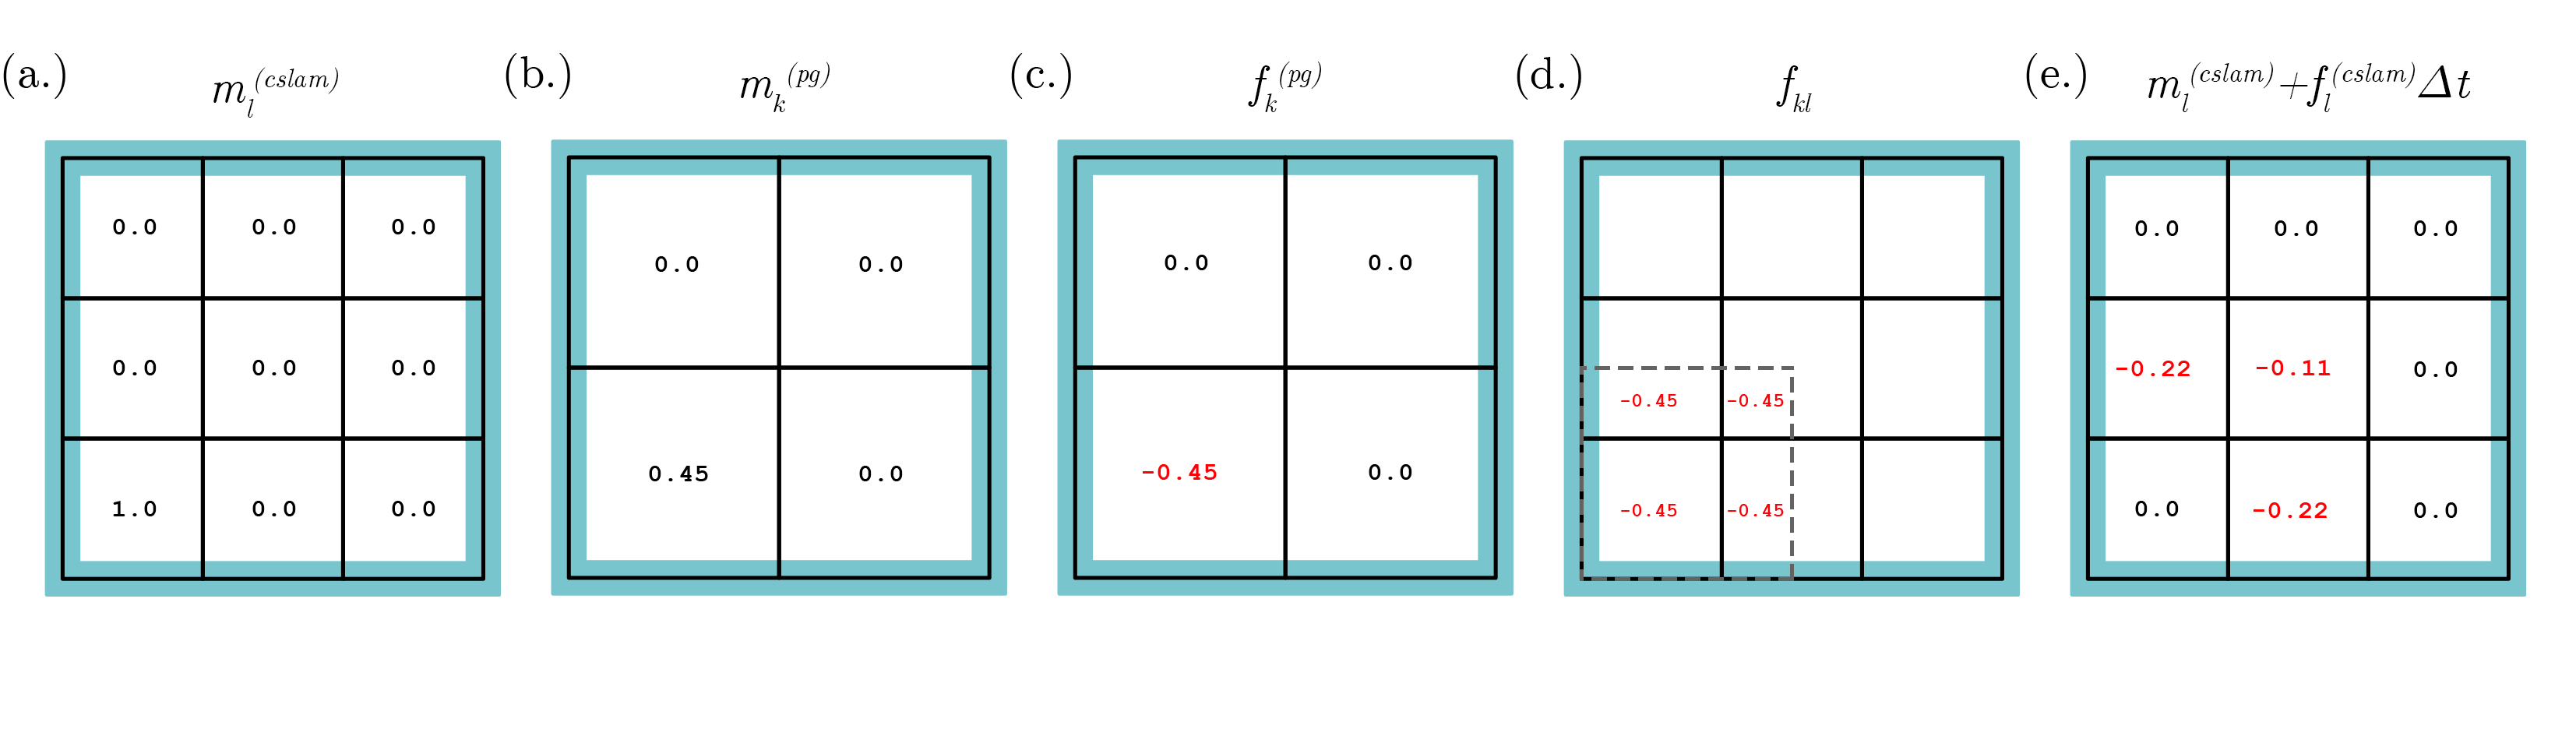
\includegraphics[width=30pc,angle=0]{figs/alg-schematic.png}\\
\end{center}
\caption{Make captions stand-alone while being concise}
\label{fig:alg-schematic}
\end{figure}

Even if one could derive a reversible map for mapping $\Delta p$ from physics grid to the CSLAM grid there could still be problems with driving mixing ratios negative on the CSLAM grid (we refer to this as the `negativity problem'). This problem is depicted schematically in Figure~\ref{fig:alg-schematic}. Consider a single element of CSLAM control volumes, containing only a single cell with mixing ratio $1.0$, and $0.0$ everywhere else ($m_l$; Figure ~\ref{fig:alg-schematic}a). Assume that the mixing ratios mapped to the $pg2$ grid ($m_k$; Figure~\ref{fig:alg-schematic}b) results in a negative tracer increment from the physics ($f_k$; Figure~\ref{fig:alg-schematic}c). The non-zero values of the increments for $pg2$ areas overlapping CSLAM grid cells originally containing a mixing ratio of zero ($f_{k,l}$; Figure~\ref{fig:alg-schematic}d), are driven negative by the mapped increment (Figure~\ref{fig:alg-schematic}e). 

The negativity issue could be avoided if one remaps the physics updated state instead of mapping increments/tendencies. In that case a shape-preserving filter will make sure that the state on the CSLAM grid is not negative (and does not overshoot). That said, if physics does not change the state and it is mapped back to the CSLAM grid then spurious tendencies (proportional to the errors introduced by mapping state from the CSLAM grid to the physics grid and back again) are introduced. Hence it is advantageous to map increments/tendencies since any reasonable algorithm will preserve a zero function.

%In the $pg2$ configuration, mapping the fields to and from the quadrature grid and $pg2$ grid is identical to that described in H18. As discussed above above, in mapping to the physics grid, CAM-SE's Lagrange basis functions are integrated over the $pg2$ control volumes to provide the physics with a volume averaged state. The procedure is accurate to machine precision, conserves thermal energy and dry air mass, and is consistent (i.e., the mapping preserves a constant). The reverse mapping, from the physics grid to the quadrature grid, is done using a tensor-product Lagrange interpolation (see Appendix A in H18). The Lagrange interpolation is consistent, conserves dry air mass ({\color{red}{Peter, is this true?}}), but does not conserve thermal energy. Errors arising from the lack of energy conservation were estimated to be small; about two orders of magnitude less than the energy dissipation due to the dynamical core alone.

%The semi-Lagrangian advection of tracers in our $pg2$ configuration is solved on the CSLAM grid. 





%Interpolation: Traditional Lagrange interpolate of the mixing ratio increment would preserve a constant and could be made shape-preserving using {\em{ad hoc}} filters \citep[e.g.][]{BC2002MWR} but will not inherently preserve mass increment and suffers from the `negativity problem' described above.

As illustrated above a standard remapping method will NOT simultaneously satisfy 1-4 and hence a new algorithm has been derived.
\subsection{Algorithm}
The problem is how to map the mass-tendency $f^{(pg)}\Delta A^{(pg)}$ to the CSLAM cells that overlap with $\Delta A^{(pg)}$; these exchange grid cells we refer to as $A_{k\ell}$. To maintain shape-preservation and to avoid the negativity problem it advantageous to define a mass excess function $\Delta m_{k\ell}^{(excess)}$ which is the amount of mixing ratio that can be removed without producing new extrema in $m_{k\ell}$
\begin{equation}
\Delta m^{(excess)}_{k\ell}=\langle m\rangle_{k\ell}-m^{(min)},
\end{equation}
where $\langle m\rangle_{k\ell}$ is a higher-order representation of the mixing ratio representation over each overlap area computed during the mapping of tracer mass to from the CSLAM grid to the physics grid (see equations \eqref{eq:mp} and \eqref{eq:mp2}). 

The maximum amount of mass that we can remove from the CSLAM cells overlapping with the $k$th physics grid cell is
\begin{equation}
\sum_\ell \Delta m^{(excess)}_{k\ell}\langle \Delta p\rangle_{k\ell} \delta A_{k\ell}.
\end{equation}
We distribute the physics mass-forcing (assuming $f^{(pg)}<0$) according to the mass excess in each overlap area by solving this equation for $\gamma_k$
\begin{equation}
\Delta A_k^{(pg)}\Delta p_k^{(pg)}f^{(pg)}=\gamma_k \sum_\ell \Delta m^{(excess)}_{k\ell}\langle \Delta p\rangle_{k\ell} \delta A_{k\ell},
\end{equation}
and add mass increment {\color{red}{[check signs!]}}
\begin{equation}
\gamma_k \Delta m^{(excess)}_{k\ell}\langle \Delta p\rangle_{k\ell} \delta A_{k\ell},
\end{equation}
to the $\ell$th CSLAM cell state $m^{(c)}\Delta A^{(nc)}_\ell \Delta p^{(nc)}_\ell$. This is a well-posed problem since physics can not remove more mass than is available; hence the negativity problem is avoided. Mass is conserved by design and shape-preservation is obtained by using the excess function.

If the physics increment is positive (assuming $f^{(pg)}<0$) we define a `lack' function
\begin{equation}
\Delta m^{(lack)}_{k\ell}=\langle m\rangle_{k\ell}-m^{(max)},
\end{equation}
and solve
\begin{equation}
\Delta A_k^{(pg)}\Delta p_k^{(pg)}f^{(pg)}=\gamma_k \sum_\ell \Delta m^{(lack)}_{k\ell}\langle \Delta p\rangle_{k\ell} \delta A_{k\ell},
\end{equation}
for $\gamma_k$ and follow the same procedure as for mass excess. Since positive and negative forcing is treated in exactly the same way, linear correlations are preserved. With the definition of the excess/lack function linear correlations would not be preserved; for example, if one would prevent negative values and not do anything about overshoots then linear correlations would not be preserved.

%Similarly we define a mass lack function

%which is the maximum amount of mixing ratio that can be added without creating new maxima.

{\color{red}{mention why the problem is well-posed}}
